\documentclass{beamer}

\usepackage[utf8]{inputenc}
\usepackage{braket}
\usepackage{url}

\graphicspath{{./images/}}

\usetheme{Copenhagen}
\setlength{\parskip}{0.5em}

\title{Quantum Criptograhy}
\subtitle{With a look at Quantum Key Distribution}
\author{Michele Beretta}
\institute{UniBG
  \\ \url{https://github.com/micheleberetta98/qkd-presentation}
}
\date{2021}

\begin{document}
  \frame{\titlepage}

  \AtBeginSection[]{
    \begin{frame}
      \frametitle{Table of Contents}
      \tableofcontents[currentsection]
    \end{frame}
  }

  \section{Introduction}
  \subsection{Basics}
  \begin{frame}
    \frametitle{The Qubit}
    The \textit{bit} is the fundamental concept of classical computation - it can be either $0$ or $1$.

    In a quantum world, where \textit{superposition of states} is a thing, we use an analogous concept -
    the \textit{quantum bit}, or \textbf{qubit}.

    A qubit can be in any \textit{linear combination} of two base states.
  \end{frame}
  \begin{frame}
    \frametitle{The Qubit}
    A classical bit is like a coin - either \textit{head} or \textit{tail}.

    A qubit can be both \textit{head} or \textit{tail} at the same time - that is, until observed.

    Observing a qubit makes it \textit{decay} in one of the base states. Hence, measurement
    \textit{changes} the real world.
  \end{frame}
  \begin{frame}
    \frametitle{Making a Quantum Computer}
    Making a qubit is hard - for example, nuclear spin can be mantained for long, but it's hard to measure.

    A good quantum computer has to be \textit{well isolated}, but its qubits have to be \textit{accessible}
    in order to be manipulated.
  \end{frame}
  
  \subsection{Notation}
  \begin{frame}
    \frametitle{A Mathematical Representation}
    \begin{block}{Qubit}
      Given two states $\ket{0}$ and $\ket{1}$ a qubit is defined as
      \begin{equation*}
        \ket{\psi} = \alpha\ket{0} + \beta\ket{1} \quad \alpha,\beta\in\mathbb C
      \end{equation*}
    \end{block}

    For our purposes, it's safe to assume $\alpha,\beta\in\mathbb R$.
  \end{frame}
  \begin{frame}
    \frametitle{Some Linear Algebra}
    A qubit can be thought as a \textit{vector} in a $2$-dimensional vector space.
    The states $\ket 0$ and $\ket 1$ are the basis of this space.

    One example could be
    \begin{equation*}
      \ket{0} = \begin{bmatrix} 1 \\ 0 \end{bmatrix},
      \quad
      \ket{1} = \begin{bmatrix} 0 \\ 1 \end{bmatrix}
      \implies
      \ket{\psi} = \begin{bmatrix} \alpha \\ \beta \end{bmatrix}
    \end{equation*}

    Some operations
    \begin{itemize}
      \item \textit{Dot product}: $\braket{\psi|\varphi}$
      \item \textit{Tensor product}: $\ket{\psi}\otimes\ket{\varphi} = \ket{\psi}\ket{\varphi}$
    \end{itemize}

    Note that $\bra{\psi} = \ket{\psi}^T$.
  \end{frame}
  \begin{frame}
    \frametitle{Measuring}
    When measuring a qubit, we can get:
    \begin{itemize}
      \item A $0$ with probability $|\alpha|^2$
      \item A $1$ with probability $|\beta|^2$
    \end{itemize}

    Since they are probabilities, it has to be
    \begin{equation*}
      |\alpha|^2 + |\beta|^2 = 1
    \end{equation*}
    Or, in other words, the qubit's state must be \textit{normalized}.
  \end{frame}
  \begin{frame}
    \frametitle{So what is a qubit?}
    \begin{block}{Mathematical Representation of a Qubit}
      A qubit is a \textit{unit vector} in a \textit{two-dimensional complex vector field}.
    \end{block}

    For example
    \begin{equation*}
      \ket\psi = \frac1{\sqrt 2}\ket0 + \frac1{\sqrt 2}\ket1
    \end{equation*}
    is a qubit that, when measured, gives either $0$ or $1$ fifty-percent of the time.
  \end{frame}
  \begin{frame}
    \frametitle{More qubits?}
    We can combine multiple qubits. For example, a 2-qubit system has four \textit{computational basis}
    \begin{equation*}
      \ket\psi = \alpha_{00}\ket{00} + \alpha_{01}\ket{01} + \alpha_{10}\ket{10} + \alpha_{11}\ket{11}
    \end{equation*}

    In this system, a qubit can be in a superposition on $4$ states.

    In general, if we have $n$ qubits, then the system can be in a superposition of $2^n$ states.
  \end{frame}
  \begin{frame}
    \frametitle{Gates}
    How do we modify qubits? With \textit{quantum gates}.
    \begin{block}{Quantum Gate}
      A quantum gate is a \textit{complex matrix} which must be unitary.
    \end{block}

    For example, the \textbf{NOT} gate is defined as
    \begin{equation*}
      X = \begin{bmatrix}
        0 & 1 \\ 1 & 0
      \end{bmatrix}
      \implies
      X\begin{bmatrix}
        \alpha \\ \beta
      \end{bmatrix}
      = \begin{bmatrix}
        \beta \\ \alpha
      \end{bmatrix}
    \end{equation*}

    It's called a \textbf{NOT} gate because it inverts the probabilities of measuring $0$ and $1$.
  \end{frame}
  \begin{frame}
    \frametitle{More gates}
    Other important gates are:
    \begin{itemize}
      \item The \textbf{Z} gate, which flips the sign of the $\ket{1}$ state
      \begin{equation*}
        Z = \begin{bmatrix}
          1 & 0 \\ 0 & -1
        \end{bmatrix}
      \end{equation*}
      \item The \textbf{H} gate, or \textit{Hadamard} gate, used to bring the qubit in a superposition
      \begin{equation*}
        H = \frac1{\sqrt 2}\begin{bmatrix}
          1 & 1 \\ 1 & -1
        \end{bmatrix}
      \end{equation*}
    \end{itemize}  
  \end{frame}
  \begin{frame}
    \frametitle{A multi-qubit gate: CNOT}
    A \textit{controlled-not} or \textbf{CNOT} gate is a two-qubit input gate, the \textit{control} qubit
    and the \textit{target} qubit.

    The target qubit is flipped if the control qubit is set to $1$. Its matrix is
    \begin{equation*}
      U_{CN} = \begin{bmatrix}
        1 & 0 & 0 & 0 \\
        0 & 1 & 0 & 0 \\
        0 & 0 & 0 & 1 \\
        0 & 0 & 1 & 0
      \end{bmatrix}
    \end{equation*}

    And its effect is such that
    \begin{equation*}
      \ket{A,B} \to \ket{A,B\oplus A}
    \end{equation*}

    Where $\oplus$ is addition modulo two.
  \end{frame}

  \subsection{No-cloning theorem}
  \begin{frame}
    \frametitle{Can we copy a qubit?}
    If we measure a qubit we destroy its superposition - but can we copy the qubit itself?
    
    The answer is \textbf{no}. It is impossible to make a copy of an unknown quantum state.
  \end{frame}
  \begin{frame}
    \frametitle{Proof/1}
    It's a proof by absurd.

    Suppose it exists a copying machine that copies a qubit $\ket{\psi}$ into another qubit $\ket{s}$.
    The initial state of this machine is
    \begin{equation*}
      \ket{\psi} \otimes \ket{s}
    \end{equation*}
    So there is a unitary evolution $U$ that actually does the copying procedure, ideally
    \begin{equation*}
      \ket{\psi} \otimes \ket{s} \xrightarrow{U} \ket{\psi} \otimes \ket{\psi}
    \end{equation*}
    Now, given two particular states $\ket{\psi}$ and $\ket{\varphi}$, we have
    \begin{align*}
      U(\ket{\psi}\otimes\ket{s}) &= \ket{\psi}\otimes\ket{\psi} \\
      U(\ket{\varphi}\otimes\ket{s}) &= \ket{\varphi}\otimes\ket{\varphi}
    \end{align*}
  \end{frame}
  \begin{frame}
    \frametitle{Proof/2}
    Taking the inner product of these two equations gives us
    \begin{equation*}
      \braket{\psi|\varphi} = \left(\braket{\psi|\varphi}\right)^2
    \end{equation*}
    But $x = x^2$ has only two solutions - $0$ and $1$, which means
    \begin{equation*}
      \braket{\psi|\varphi} = 0 \vee \braket{\psi|\varphi} = 1
    \end{equation*}
    So $\ket{\psi} = \ket{\varphi}$ or $\ket{\psi}$ and $\ket{\varphi}$ are orthogonal.

    Hence we can only clone orthogonal states, making general quantum cloning impossible.
  \end{frame}

  \section{Quantum Cryptography}
  \subsection{Why}
  \begin{frame}
    \frametitle{Why do we care about this?}
    Because quantum computers could be capable of a lot of things.
    
    Namely, efficiently perform some tasks that \textit{are not feasible on a classical computer}.

    In particular, \textbf{public key cryptography} is based on the infeasibility of
    some problems, such as prime factorization or discrete logarithm.
  \end{frame}
  \begin{frame}
    \frametitle{Fast prime factorization}
    For example, finding the prime factorization of an $n$-bit integer requires
    \begin{equation*}
      \exp{\Theta\left(n^{\frac13}\log^{\frac23}n\right)}
    \end{equation*}
    operations using the \textit{number field sieve}.

    A quantum algorithm can accomplish the same task using
    \begin{equation*}
      O\left(n^2\log n \log\log n\right)
    \end{equation*}
    operations - so it's \textit{exponentially faster}.

    The demonstration is quite lengthy, but can be found in
    \cite{nielsen-chuang} or in \cite{de-wolf}.
  \end{frame}

  \subsection{Quantum Key Distribution}
  \begin{frame}
    \frametitle{Private Key Cryptography}
    In a private key cryptosystem, if Alice and Bob wish to exchange information they
    both must have a \textit{matching key}, used to encrypt and decrypt the message.

    As long as the keys are truly secret, this method is provably secure.

    The problem is the \textit{secure distribution}
    of the keys.
  \end{frame}
  \begin{frame}
    \frametitle{Quantum Key Distribution (QKD)}
    It's a \textit{provably secure} protocol by which \textit{private keys} can be created
    between two parties over a \textit{public channel}, exchanging qubits.

    An external observer (Eve) cannot gain any information from the qubits
    transmitted without disturbing the state, because
    \begin{enumerate}
      \item<1-> Qubits cannot be copied (no-cloning theorem)
      \item<2-> Measurement changes the data itself
    \end{enumerate}
  \end{frame}
  \begin{frame}
    \frametitle{The BB84 Protocol/1}
    Suppose Alice and Bob want to distill a shared secret key
    
    Alice has two strings $a$ and $b$ of $(4+\delta)n$ bits.
    She encodes them as a block of $(4+\delta)n$ qubits
    \begin{equation*}
      \ket{\psi} = \bigotimes_{k=1}^{(4+\delta)n} \ket{\psi_{a_kb_k}}
    \end{equation*}
    where $a_k$ is the $k^\text{th}$ bit of $a$ (similarly for $b$).
  \end{frame}

  \begin{frame}
    \frametitle{The BB84 Protocol/2}
    So every qubit is one of these four states
    \begin{align*}
      \ket{\psi_{00}} &= \ket{0} & \ket{\psi_{10}} &= \ket{1} \\
      \ket{\psi_{01}} &= \ket{+} = \frac{\ket0 + \ket1}{\sqrt2} &\ket{\psi_{11}} &= \ket{-} = \frac{\ket0 - \ket1}{\sqrt2}
    \end{align*}

    We can think of these as qubits encoded in one of two basis - $X$ or $Z$ - based
    on the value of the bit $b_k$:
    \begin{itemize}
      \item $b_k = 0 \implies 0 \to \ket0, 1 \to \ket1$
      \item $b_k = 1 \implies 0 \to \ket{+}, 1 \to \ket{-}$
    \end{itemize}
  \end{frame}

  \begin{frame}
    \frametitle{The BB84 Protocol/3}
    If Eve is eavesdropping, then Bob receives a ``disturbed'' version of the qubits.

    When Bob receives the qubits, he announces it and then
    measures each qubit in basis $X$ or $Z$, based on a $(4+\delta)n$ bits
    string $b'$, created randomly. Let's call the measurement result $a'$.
  \end{frame}

  \begin{frame}
    \frametitle{The BB84 Protocol/4}
    Alice publicly transmits $b$, and Alice and Bob discard any bits where Bob measured
    a different basis than Alice prepared.

    With high probability, there are at least $2n$ bit left (if not, abort). Let's keep only the first $2n$ bits.

    Alice chooses a subset of $n$ bits as a check, and tells Bob which bits she selected.
    
    
    They both compare these, and if more than an acceptable number of bits disagree the protocol is aborted.
    Otherwise, they have the key!
  \end{frame}

  \begin{frame}
    \frametitle{The BB84 Protocol - summary}
    \begin{enumerate}
      \item Alice prepares $(4 + \delta)n$ random data bits - $a$
      \item Alice randomly chooses $(4 + \delta)n$ random base bits - $b$
      \item She encodes each data bit $a_i$ as $(\ket0, \ket1)$ if $b_i = 0$, or as $(\ket+, \ket-)$ if $b_i = 1$
      \item She sends the qubits to Bob
      \item Once received, Bob measures each qubit in a random base ($X$ or $Z$)
      \item Alice announces $b$
      \item Alice and Bob keep only the bits measured in the same bases, and max $2n$ bits
      \item Alice chooses $n$ bits as a check and tells Bob which ones she selected
      \item They both compare these bits, and if they match then the remaining bits are the key
    \end{enumerate}  
  \end{frame}

  \begin{frame}
    \frametitle{Quick demo}
  
    \begin{center}
      \begin{figure}[H]
        \centering
        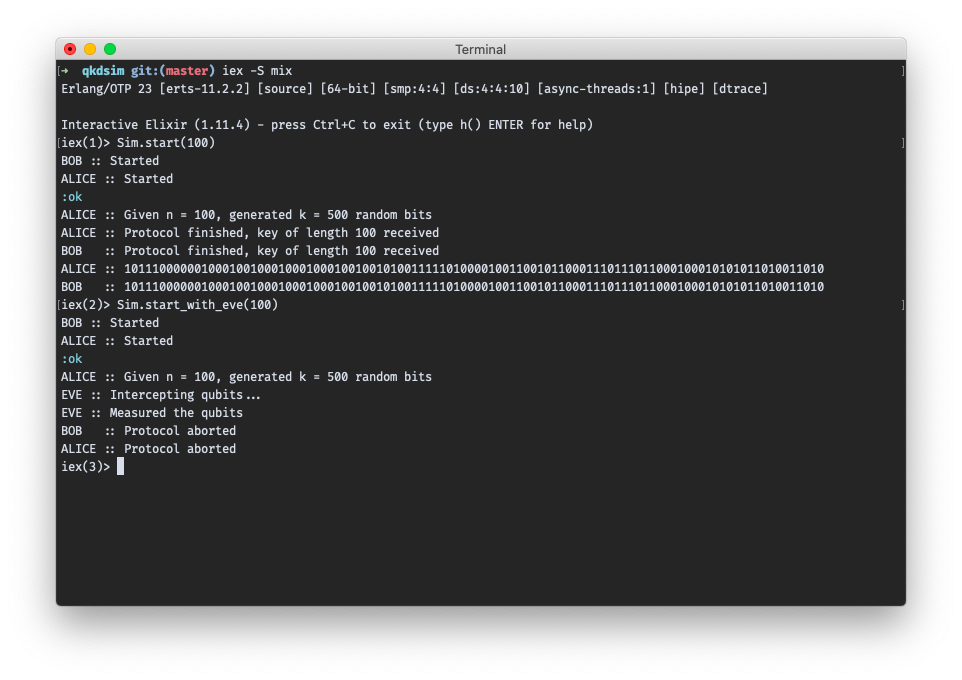
\includegraphics[width=0.8\linewidth]{qkd-bb84-elixir.png}
      \end{figure}

      \small{Code available at \url{https://github.com/micheleberetta98/qkd-sim}}
    \end{center}
  
  \end{frame}

  \subsection{In real life}
  \begin{frame}
    \frametitle{But does any of this work?}
    Yes, Quantum Key Distribution has already been tested in real life.
    For example
    \begin{itemize}
      \item In 2015 the Unversity of Geneva and Corning Inc. achieved a secret key
            rate of $12.7 \mathrm{kbit/s}$ over $307 \mathrm{km}$ \cite{qkd}
      \item In 2017 the Institute for Quantum Compuing and the University of Waterloo (Canada) achieved
            quantum key distribution between a ground transmitter and a moving aircraft \cite{airborne}
    \end{itemize}
  \end{frame}
  
  \section*{}
  \begin{frame}{References and further reading}
    \nocite{*}
    \bibliographystyle{alpha}
    \bibliography{bibliography}
  \end{frame}

\end{document}